% !TEX root = handbook-physics.tex
%!TEX TS-program = pdflatex
%!TEX encoding = UTF-8 Unicode

\chapter{Second Law Of Thermodynamics}
\label{ch-11}


\section{Cycles. The Carnot Cycle}
\label{sec-11.1}

\subsection{}\label{11.1.1}A \emph{cycle} is a succession of thermodynamic processes \ssect{8.3.7} as a result of which the system returns to its initial state. In $pV$, $pT$ and other thermodynamic diagrams, equilibrium cycles \ssect{8.3.7} are represented in the form of closed curves, because two identical states, the beginning and end of the cycle, correspond to the same point of the diagram. A thermodynamic system that accomplishes a cycle and exchanges energy with other bodies is called the \emph{working medium}, or \emph{substance}. This medium is usually a gas.

\subsection{}\label{11.1.2} The arbitrary equilibrium cycle $C_{1}aC_{2}bC_{1}$ \figr{fig-11-01}, using an ideal gas, can be divided into the process of expansion of the gas from state $C_{1}$, to state $C_{2}$ (curve $C_{1}aC_{2}$) and the process of compressing the gas from state $C_{2}$ to state $C_{1}$ (curve $C_{2}bC_{1}$). In expansion the gas does positive work $W_{1}$ measured by the area under the curve $C_{1}aC_{2}$ (the area of the figure $V_{1}C_{1}C_{2}V_{2}$ see Sect. \ssect{9.4.2}. The gas is compressed by external forces that do positive work $W_{2}' = -W_{2}$ measured by the area under the curve $C_{1}bC_{2}$ (the area of the figure $V_{1}C_{1}bC_{2}V_{2}$). Since $W_{1}> W_{2}'$ (\figr{fig-11-01}), the gas does the \emph{positive} work $W = W_{1} + W_{2} = W_{1} — W_{2}'$ in the cycle. This work is measured by the hatched area, bounded by the curve $C_{1}aC_{2}bC_{1}$ of the process.


\begin{figure}[!ht]
\centering
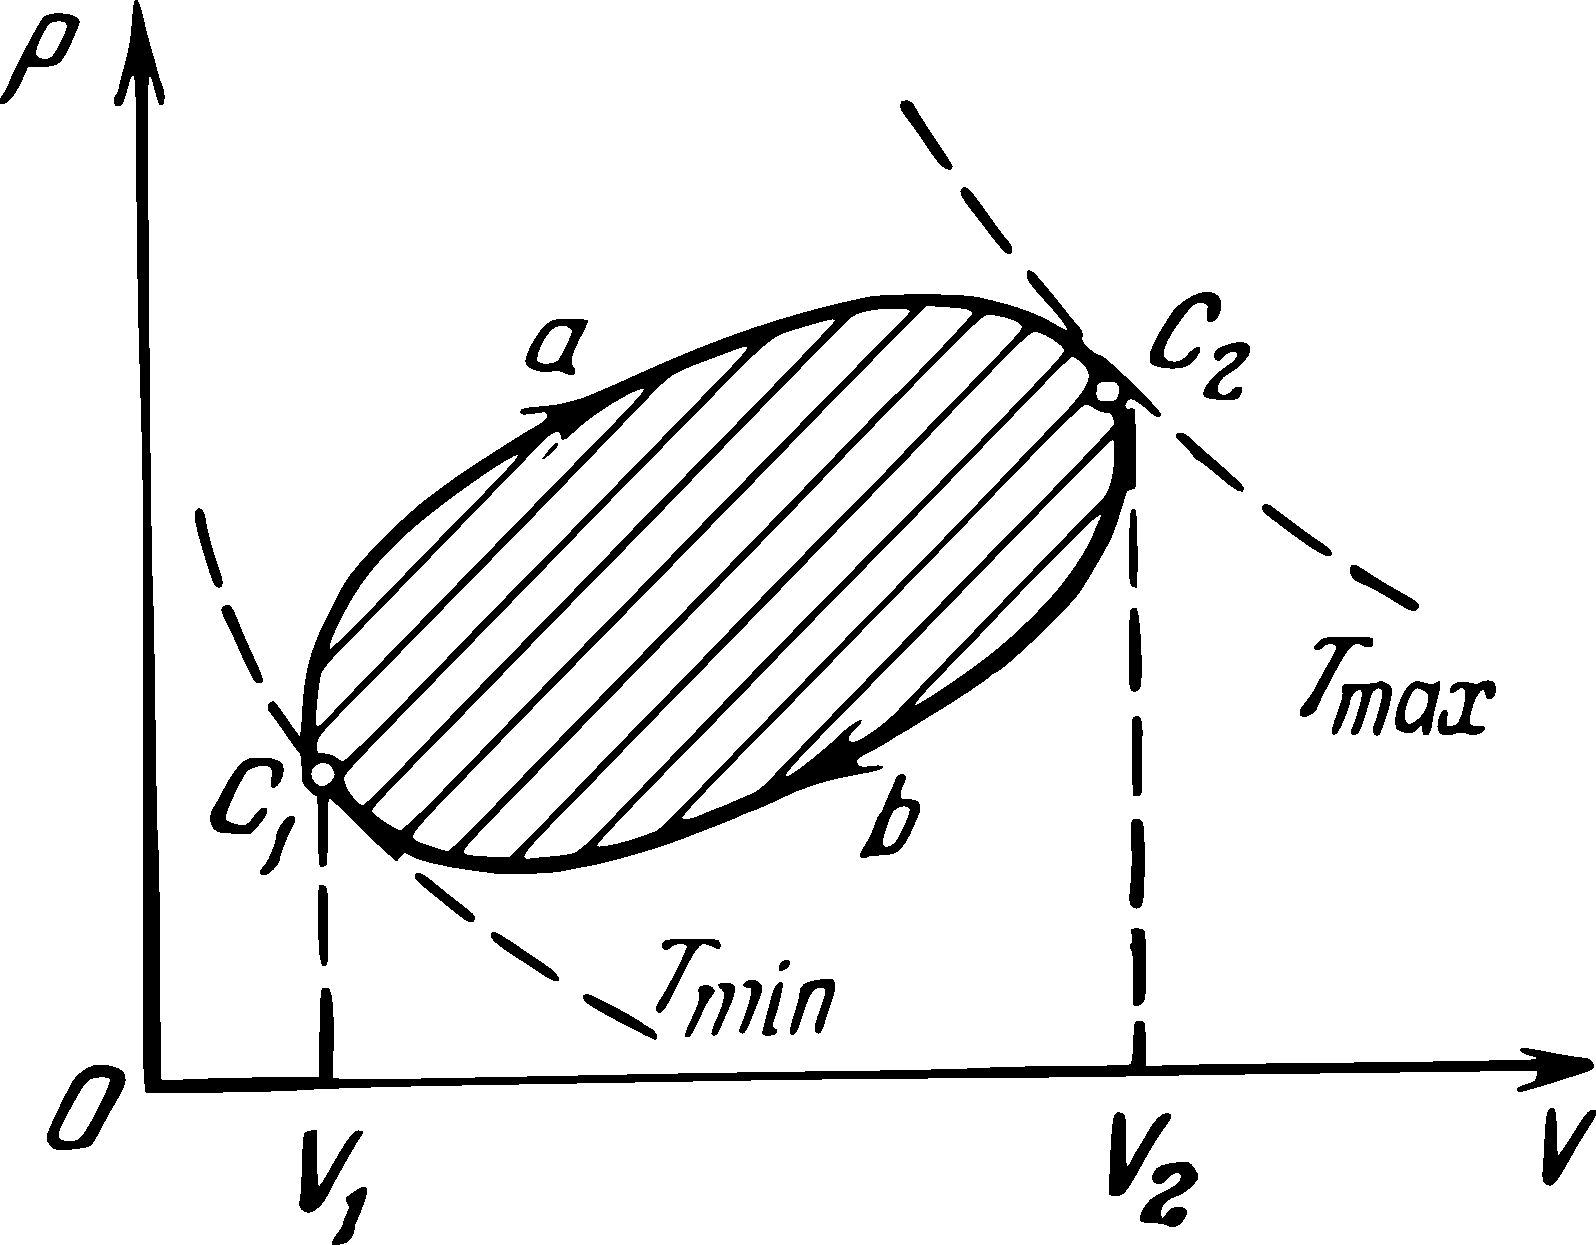
\includegraphics[width=0.6\textwidth]{figs/ch-11/fig-11-01.pdf}
\caption{An arbitrary equilibrium of a cycle.}
\label{fig-11-01}
\end{figure}

\subsection{}\label{11.1.3} A \emph{direct cycle} is one in which the system does positive work $W =\oint p \,\dd V > 0$.In a $pV$ diagram a direct cycle is represented by a closed curve along which the working medium passes in the clockwise direction \figr{fig-11-01}. An example of a direct cycle is that accomplished by the working medium in a heat engine. In such an engine the working medium \ssect{11.1.1} receives energy in the form of heat \ssect{9.2.1} from external sources and gives a part of it up in the form of work \ssect{9.2.1} (see Sect. \ssect{11.1.5}).

\subsection{}\label{11.1.4} A \emph{reverse cycle} is one in which the system does negative work $W =\oint p \, \dd V < 0$. In a $pV$ diagram a reverse cycle is represented by a closed curve along which the working medium passes in the counterclockwise direction. An example of a re­ verse cycle is that accomplished by the working medium in a refrigerator. In such a device the working medium receives energy in the form of work and transmits energy in the form of heat from a cold body to a hotter one (see Sect. \ssect{11.1.5}). 

\subsection{}\label{11.1.5} Since the total change in the internal energy of a gas in a cycle is equal to zero \ssect{9.1.3}, the first law of thermo­ dynamics \ssect{9.3.1} for such a process is of the form
\begin{equation*}%
Q = \Delta U + W = W
\end{equation*}
where $Q$ is the total quantity of heat delivered to the gas in the cycle, and $W$ is the work done by the gas in this cycle.

In a direct cycle \ssect{11.1.3} $Q > 0$ and $A > 0$,and the gas does work owing to the heat delivered to it. In a reverse cycle \ssect{11.1.4} the work done \emph{on the gas} is $W' = -W$ (where $W > 0$) and a quantity of heat equivalent to this work is removed from the gas. 


\begin{figure}[!ht]
\centering
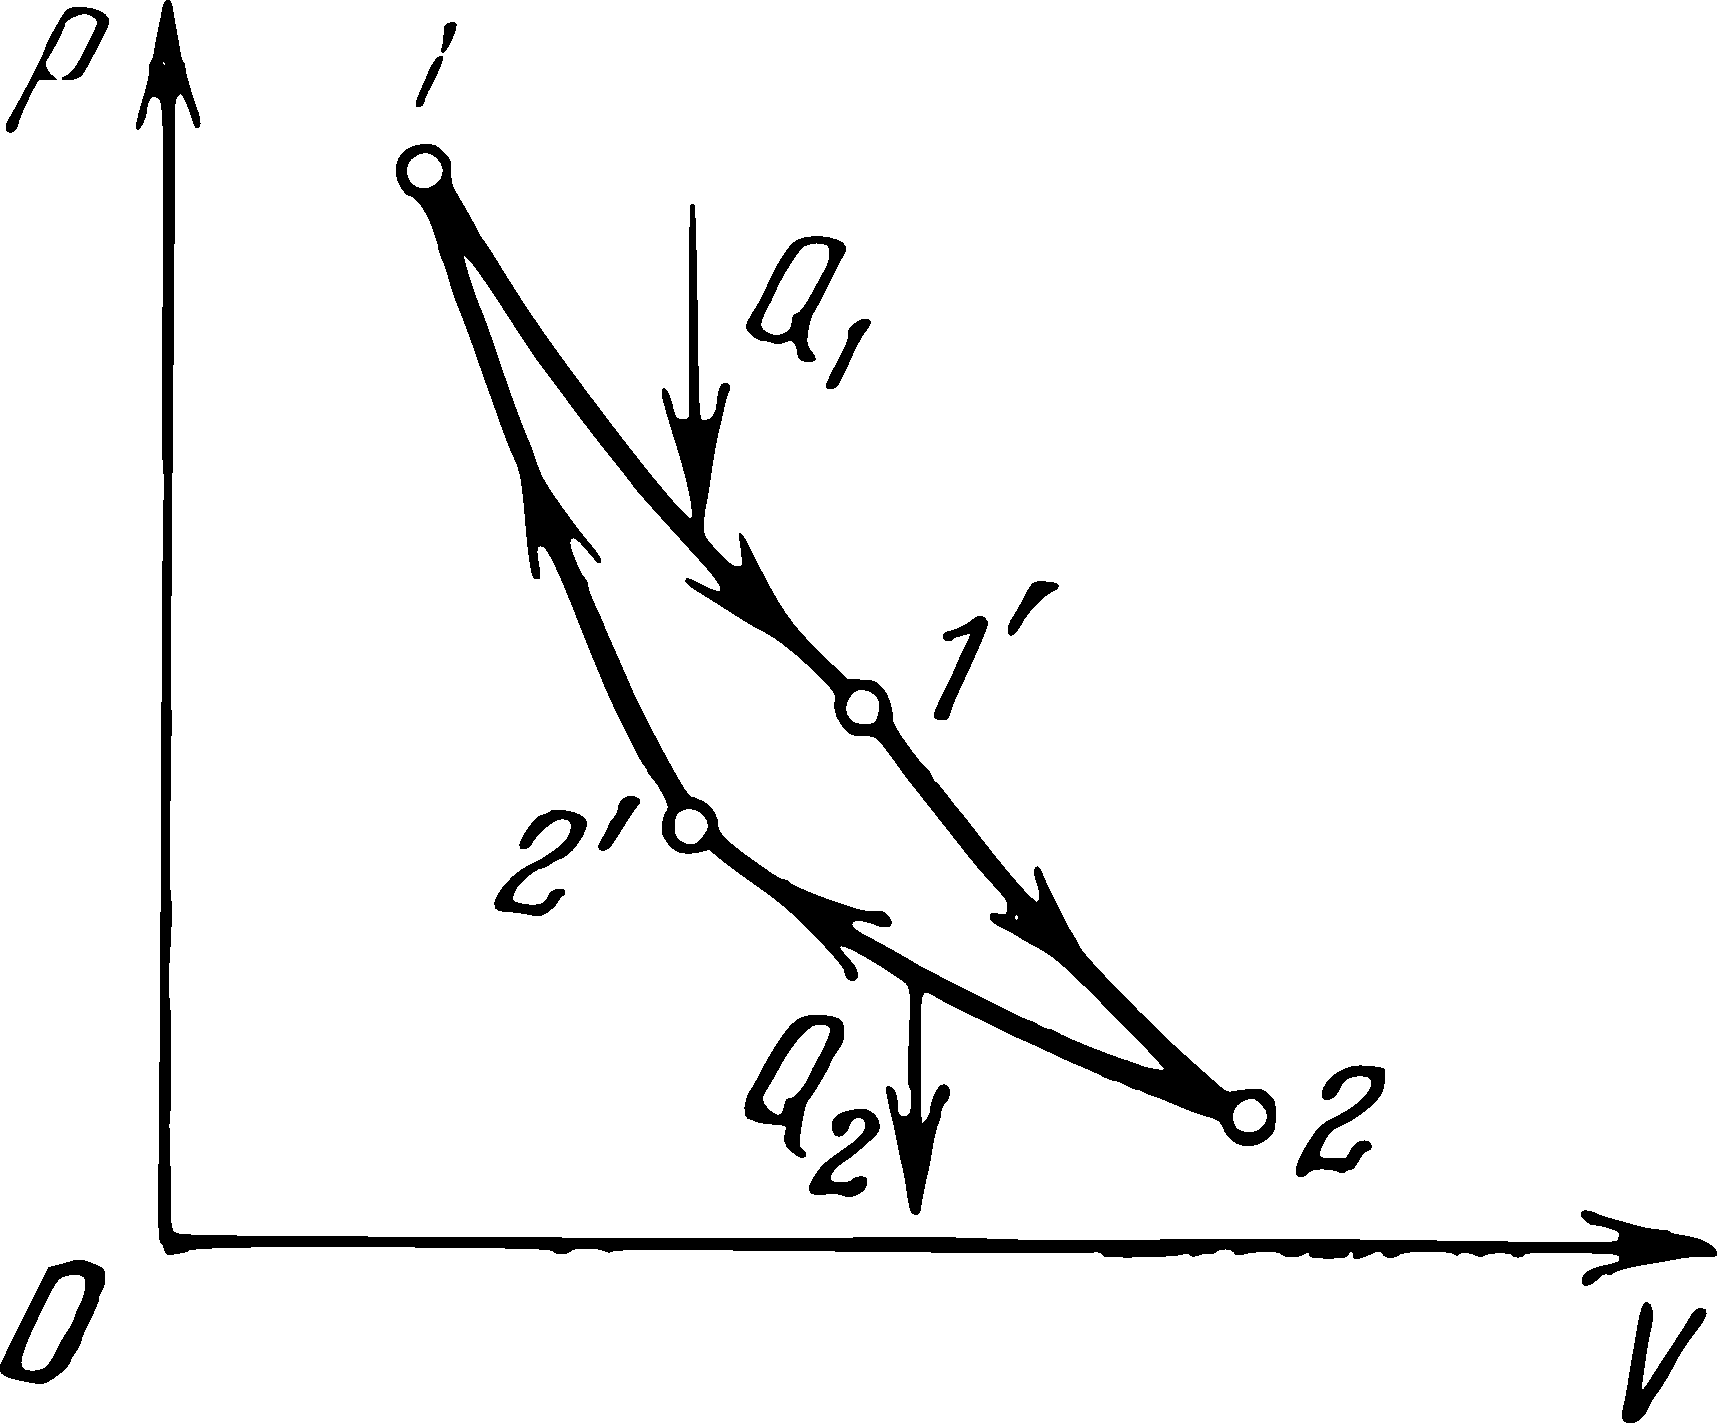
\includegraphics[width=0.5\textwidth]{figs/ch-11/fig-11-02.pdf}
\caption{The Carnot cycle.}
\label{fig-11-02}
\end{figure}


\subsection{}\label{11.1.6} The \emph{Carnot cycle} is the one shown in \figr{fig-11-02}. The \emph{direct Carnot cycle} consists of four consecutive processes: isother­mal expansion $1-1'$ at the temperature $T_{1}$ (where $T_{1}' = T_{2}$) adiabatic expansion $1'-2$, isothermal compression $2-2'$ at the temperature $T_{2}$ (where $T_{2}' = T_{2}$), and adiabatic compres­sion $2'-1$.

\subsection{}\label{11.1.7} In practice a direct Carnot cycle could be carried out by means of a gas enclosed in a vessel with a movable piston. In the process $1-1'$ the gas is in thermal contact with a \emph{heat source (heater)} at the constant temperature $T_{1}$\footnote{For instance, a large tank filled with water.}. From the heater the gas receives a certain quantity of heat $Q_{1}$ (where $Q_{1} > 0$). It is assumed that this does not change the temperature of the heater. This is possible, strictly speaking, only if the heater has an infinite heat capacity. In the process $1'-2$ the gas is thermally isolated and its expansion is adiabatic\footnote{ For instance, the cylinder with the gas is covered with a thick layer of felt.} \ssect{9.5.10}. In the process $2-2'$ the gas is brought into thermal contact with a \emph{cooler (heat sink)} having the constant temperature $T_{2}$ (where $T_{2} < T_{1}$). Here the gas is isothermically compressed and gives off the quantity of heat $—Q_{2}$ to the cooler (assuming that $Q$ is the quantity of heat received by the gas from the cooler). The heat capacity of the cooler is assumed to be infinitely high. In the state $2'$ the gas is again thermally insulated and contracts adiabatically to its initial state $1$.

\subsection{}\label{11.1.8} The work done by the gas in an equilibrium (8.3.7) direct Carnot cycle is
\begin{equation*}%
W = Q = Q_{1} + Q_{2} = Q_{1} - \abs{Q_{2}}
\end{equation*}
It is evident from the equation that $W< Q_{1}$ i, i.e. the work done by the working medium \ssect{11.1.1} in the Carnot cycle is less than the energy received from the heater by the amount of energy given up to the cooler in the form of heat. This is valid for an arbitrary process: the work $W$ done in the cycle is always less than the sum $Q_{\textrm{del}}$ of all the quantities of heat delivered to the working medium from heaters. 

The operation of heat engines is based on the direct Carnot cycle.

\subsection{}\label{11.1.9} The \emph{thermal efficiency} $\eta$ is the ratio of the work $W$ done by the working medium in a direct cycle to the sum $Q_{\textrm{del}}$ of all quantities of heat delivered in this cycle to the working medium by heaters:
\begin{equation*}%
\eta = \frac{W}{Q_{\textrm{del}}}
\end{equation*}
The quantity $\eta$ characterizes the economy of operation of a heat engine.

\subsection{}\label{11.1.10} The thermal efficiency of a direct equilibrium Carnot cycle carried out with an ideal gas is
\begin{equation*}%
\eta_{c} = \frac{Q_{1}+Q_{2}}{Q_{1}} = \frac{T_{1}-T_{2}}{T_{1}} = 1 - \frac{T_{2}}{T_{1}}
\end{equation*}
The value of $\eta_{c}$ depends only on the ratio of the temperatures of the cooler $(T_{2})$ and the heater $(T_{1})$.

\begin{figure}[!ht]
%\begin{wrapfigure}{r}{0.5\linewidth}
\centering
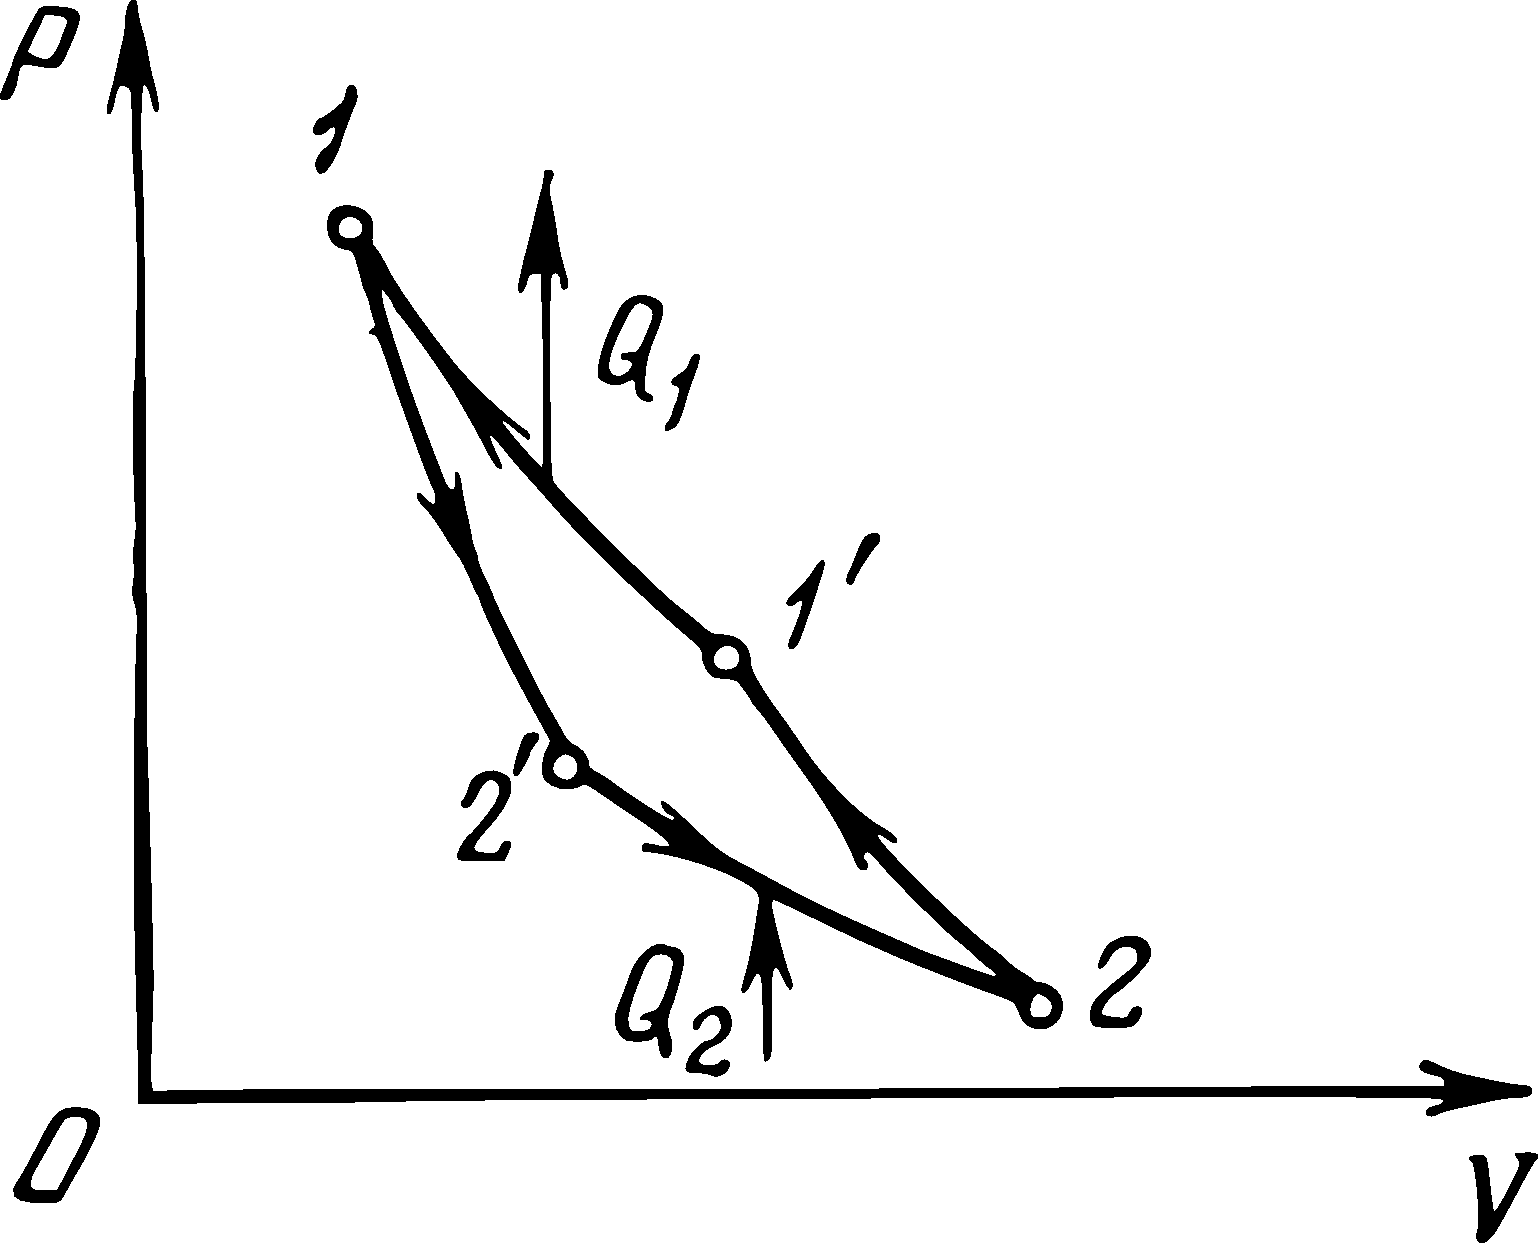
\includegraphics[width=0.5\textwidth]{figs/ch-11/fig-11-03.pdf}
%\input{figs/ch-03/fig-03-01}
%  \vspace{-13pt}
\caption{The reverse Carnot cycle.}
\label{fig-11-03}
\end{figure}


\subsection{}\label{11.1.11} The \emph{reverse Carnot cycle} is shown in \figr{fig-11-03}. In isothermal compression, carried out in the process $1'-1$, the quantity of heat $Q_{1}$ is removed from the gas at the temperature $T_{1}$, which remains constant. In the process of isothermal expansion $2'-2$ at the temperature $T_{2} < T_{1}$,the quantity of heat $Q_{2}$ is delivered to the gas. In the reverse Carnot cycle $Q_{1} < 0$, $Q_{2} > 0$ and the work $W$ done by the gas in one cycle is negative: $W= (Q_{1} + Q_{2}) < 0$. This conclusion is valid for any reverse cycle. If the working medium carries out a reverse cycle, energy can be transferred in the form of heat \ssect{9.2.1} from a cold body to a hotter one at the expense of the corresponding work done by external forces. This principle is used in all refrigerating devices. The less the work $W'= —W$ done by external forces to extract the quantity of heat $Q_{2}$ from a cold body, the higher the economical efficiency (coefficient of performance) of a refrigerator:
\begin{equation*}%
Q_{2} = W_{1} - Q_{1} = W - \frac{W}{\eta} = - \frac{1 - \eta}{\eta} W
\end{equation*}
where $\eta$ is the thermal efficiency of the direct cycle between the same temperatures $T_{1}$ and $T_{2}$ \ssect{11.1.3} and \ssect{11.1.4}.

